\chapter{Krav}
\label{ch:Krav}

I dette afsnit beskrives optillede krav for AutoGreen, som er opstillet ud fra opgaveformuleringen. 
På Figur \ref{fig:use_case_diagram} ses Use Case diagram over systemet. Dette giver et overblik over de funktionelle krav, der er formuleret i dokumentationen på side \pageref{P-ch:Kravspec}.

\begin{figure}[h]
\centering 
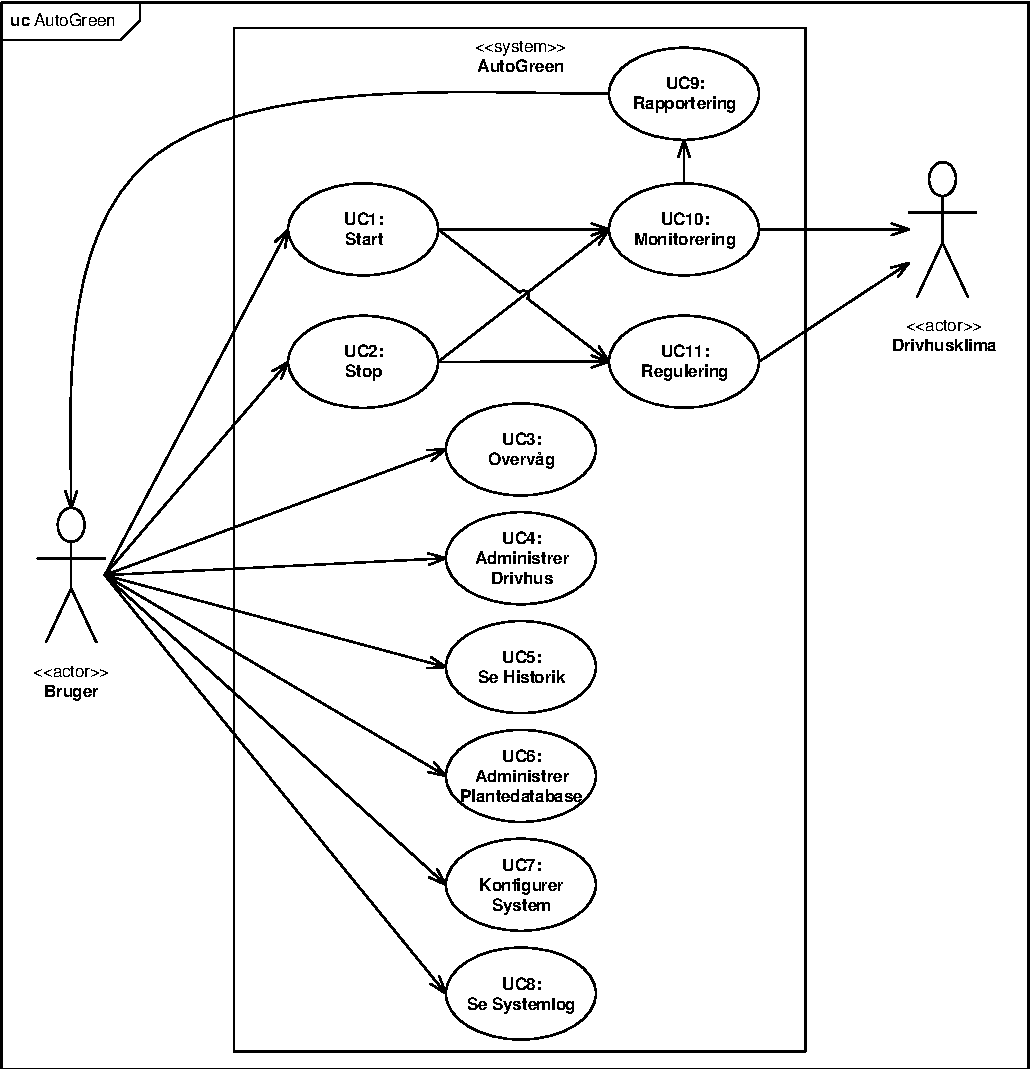
\includegraphics[width={\textwidth-1cm}, trim=0 0 0 0, clip=true] {../fig/UC_Diagram.pdf}
\caption{Use Case Diagram for AutoGreen}
\label{fig:use_case_diagram}
\end{figure}

Use Cases på billedet er kort beskrevet herunder:

\begin{itemize}

\item UC1: Start \\
Denne UC giver brugeren mulighed for at starte systemet, dvs. monitorering og regulering af drivhusklimaet.

\item UC2: Stop \\
Denne UC giver brugeren mulighed for at stoppe systemet, dvs. monitorering og regulering af
drivhusklimaet.

\item UC3: Overvåg \\
Når UC10 Monitorering er startet, vises der på brugerfladens hovedmenu alle de aktuelle måleværdier. Hvis UC11 Regulering er startet, kan værdierne for lufttemperatur og jordfugtighed være røde, hvis de ikke passer med de ønskede værdier.

\item UC4: Administrer Drivhus \\
Giver brugeren mulighed for at informere systemet om hvilke planter der er i drivhuset.

\item UC5: Se Historik \\
Giver brugeren mulighed for at se en grafisk historik over de fire målte parametre i drivhuset.

\item UC6: Administrer Plantedatabase \\
Giver brugeren mulighed for at se på planter i databasen, samt tilføje og fjerne egne planter i databasen.

\item UC7: Konfigurer System \\
Giver brugeren mulighed for at rette i systemindstillinger.

\item UC8: Se Systemlog \\
Giver brugeren mulighed for at se en liste over systemhændelser.

\item UC9: Rapportering \\
Rapporterer til brugeren ud fra de indstillinger brugeren har valgt. Dette sker ved afsendelse af e-mail til den eller de adresser som er valgt. 

\item UC10: Konfigurer System \\
Lagrer målinger af lufttemperatur, jordfugtighed, luftfugtighed og lysintensitet i en
data log.

\item UC11: Regulering \\
Regulerer temperaturen i drivhuset, vha. vinduesåbner, varmelegeme og luftcirkulation, med mindre brugeren har slået varmelegeme og/eller luftcirkulation fra.

\end{itemize}

Systemet skal have en grafisk brugerflade, der giver brugeren mulighed for at konfigurere og monitorere drivhuset. På brugerfladen skal brugeren have mulighed for at overvåge den aktuelle temperatur og bør desuden kunne se jordfugt, luftfugtighed og lysintensitet. Disse data logges og bør kunne aflæses på en graf, der viser historik for samtlige parametre. Systemet skal kunne regulere temperaturen i drivhuset på baggrund af de aktuelle parametre.\\
Baseret på brugeres præferencer kan systemet advare brugeren via e-mail, hvis systemet fejler eller klimaforholdene bliver kritiske. Til at regulere systemet skal brugeren kunne indstille systemet til at anvende varmelegeme og/eller ventilatorer til at justere klimaet. \\
AutoGreen bør have en plantedatabase, der indeholder foruddefinerede planter. Planterne kan indsættes i det virtuelle drivhus, og herefter skal systemet kunne regulere klimaet i det fysiske drivhus, så passer bedst til de(n) valgte plante(r). Brugeren skal kunne tilføje, fjerne og redigere planter, som er indsat i det virtuelle drivhus efter behov.

\clearpage